\section{简介}

\begin{figure}[H]
\centering

\includegraphics{img/logo152.jpg}
\end{figure}
小学生学习认字时,需要不断的复习。本软件收录人教版语文(一年级上册、一年级下册、二年级上册),可以按每课、开始到指定课、全册课文复习生字。可以自己增加新的生字、词、成语等。\\

官网:\url{http://www.ycorb.com/}\\

QQ交流群:816435601\\

此帮助适用于苹果iOS系统。

\section{开始}
\subsection{打开}
\begin{figure}[H]
	\centering
	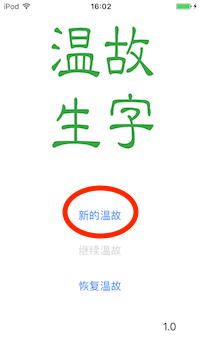
\includegraphics{img/1.png}
	\caption{首次打开}
	\label{img1}
\end{figure}
首次打开app,界面如图(\ref{img1})所示。点击“新的温故”进入数据初始化。

“恢复温故”使用请见后面\ref{restore}节。

数据初始化成功后,进入app初始默认页面,如图(\ref{img3})。
\begin{figure}[H]
	\centering
	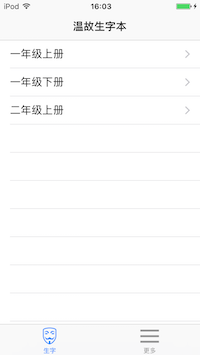
\includegraphics{img/3.png}
	\caption{默认页面}
	\label{img3}
\end{figure}

可以看到当前的语文书册列表。

\section{使用}
\subsection{复习生字}
点击“一年级上册”进入课文列表,如图(\ref{img4})
\begin{figure}[H]
	\centering
	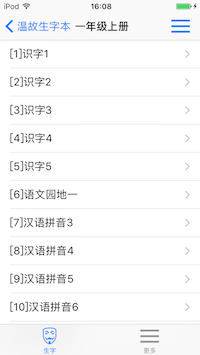
\includegraphics{img/4.png}
	\caption{课文列表}
	\label{img4}
\end{figure}

右上角,菜单有“全部复习”、“重置”。“全部复习”是复习本册语文书的所有汉字(非VIP只能复习部分),如图(\ref{img5})。“重置”是重置本册所有课程汉字到可再次复习状态。。
\begin{figure}[H]
	\centering
	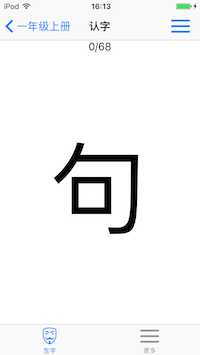
\includegraphics{img/5.png}
	\caption{所有汉字}
	\label{img5}
\end{figure}

右上角,菜单有“认识”、“不认识”、“详解”,根据实际认字情况,选择“认识”还是“不认识”。“详解”是显示当前汉字的百度汉语中的解释(需要联网)。\\

\subsection{课程复习}
回到“课程列表”,点击“识字1”,进入如图(\ref{img6})
\begin{figure}[H]
	\centering
	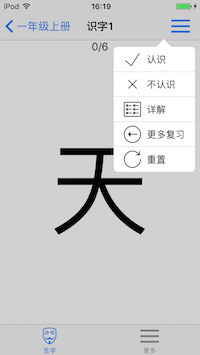
\includegraphics{img/6.png}
	\caption{复习}
	\label{img6}
\end{figure}

右上角,菜单有“认识”、“不认识”、“详解”、“更多复习”、“重置”。根据实际认字情况,选择“认识”还是“不认识”。“详解”是显示当前汉字的百度汉语中的解释(需要联网)。“更多复习”是从第一课到当前课程之间的所有汉字都在复习范围内,如图(\ref{img7})。“重置”是重置当前课程汉字到可再次复习状态。
\begin{figure}[H]
	\centering
	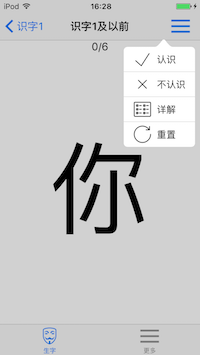
\includegraphics{img/7.png}
	\caption{复习}
	\label{img7}
\end{figure}

\subsection{我的字词}
通过“更多”---“我的字词”,增加自定义的字、词、成语,如图(\ref{img8})
\begin{figure}[H]
	\centering
	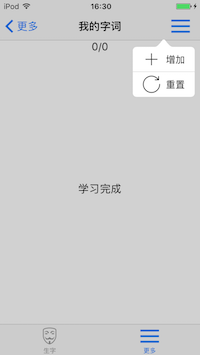
\includegraphics{img/8.png}
	\caption{我的字词}
	\label{img8}
\end{figure}

增加新字词后,如图(\ref{img9})
\begin{figure}[H]
	\centering
	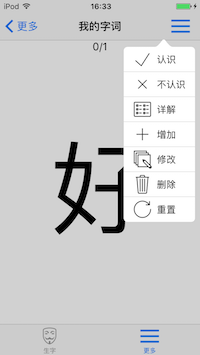
\includegraphics{img/9.png}
	\caption{我的字词}
	\label{img9}
\end{figure}

右上角菜单中“修改”为修改当前字词、“删除”为删除当前字词。其他菜单项使用同上。

